\subsection{Domänenmodell}\label{l:domänenmodell}

\begin{center}
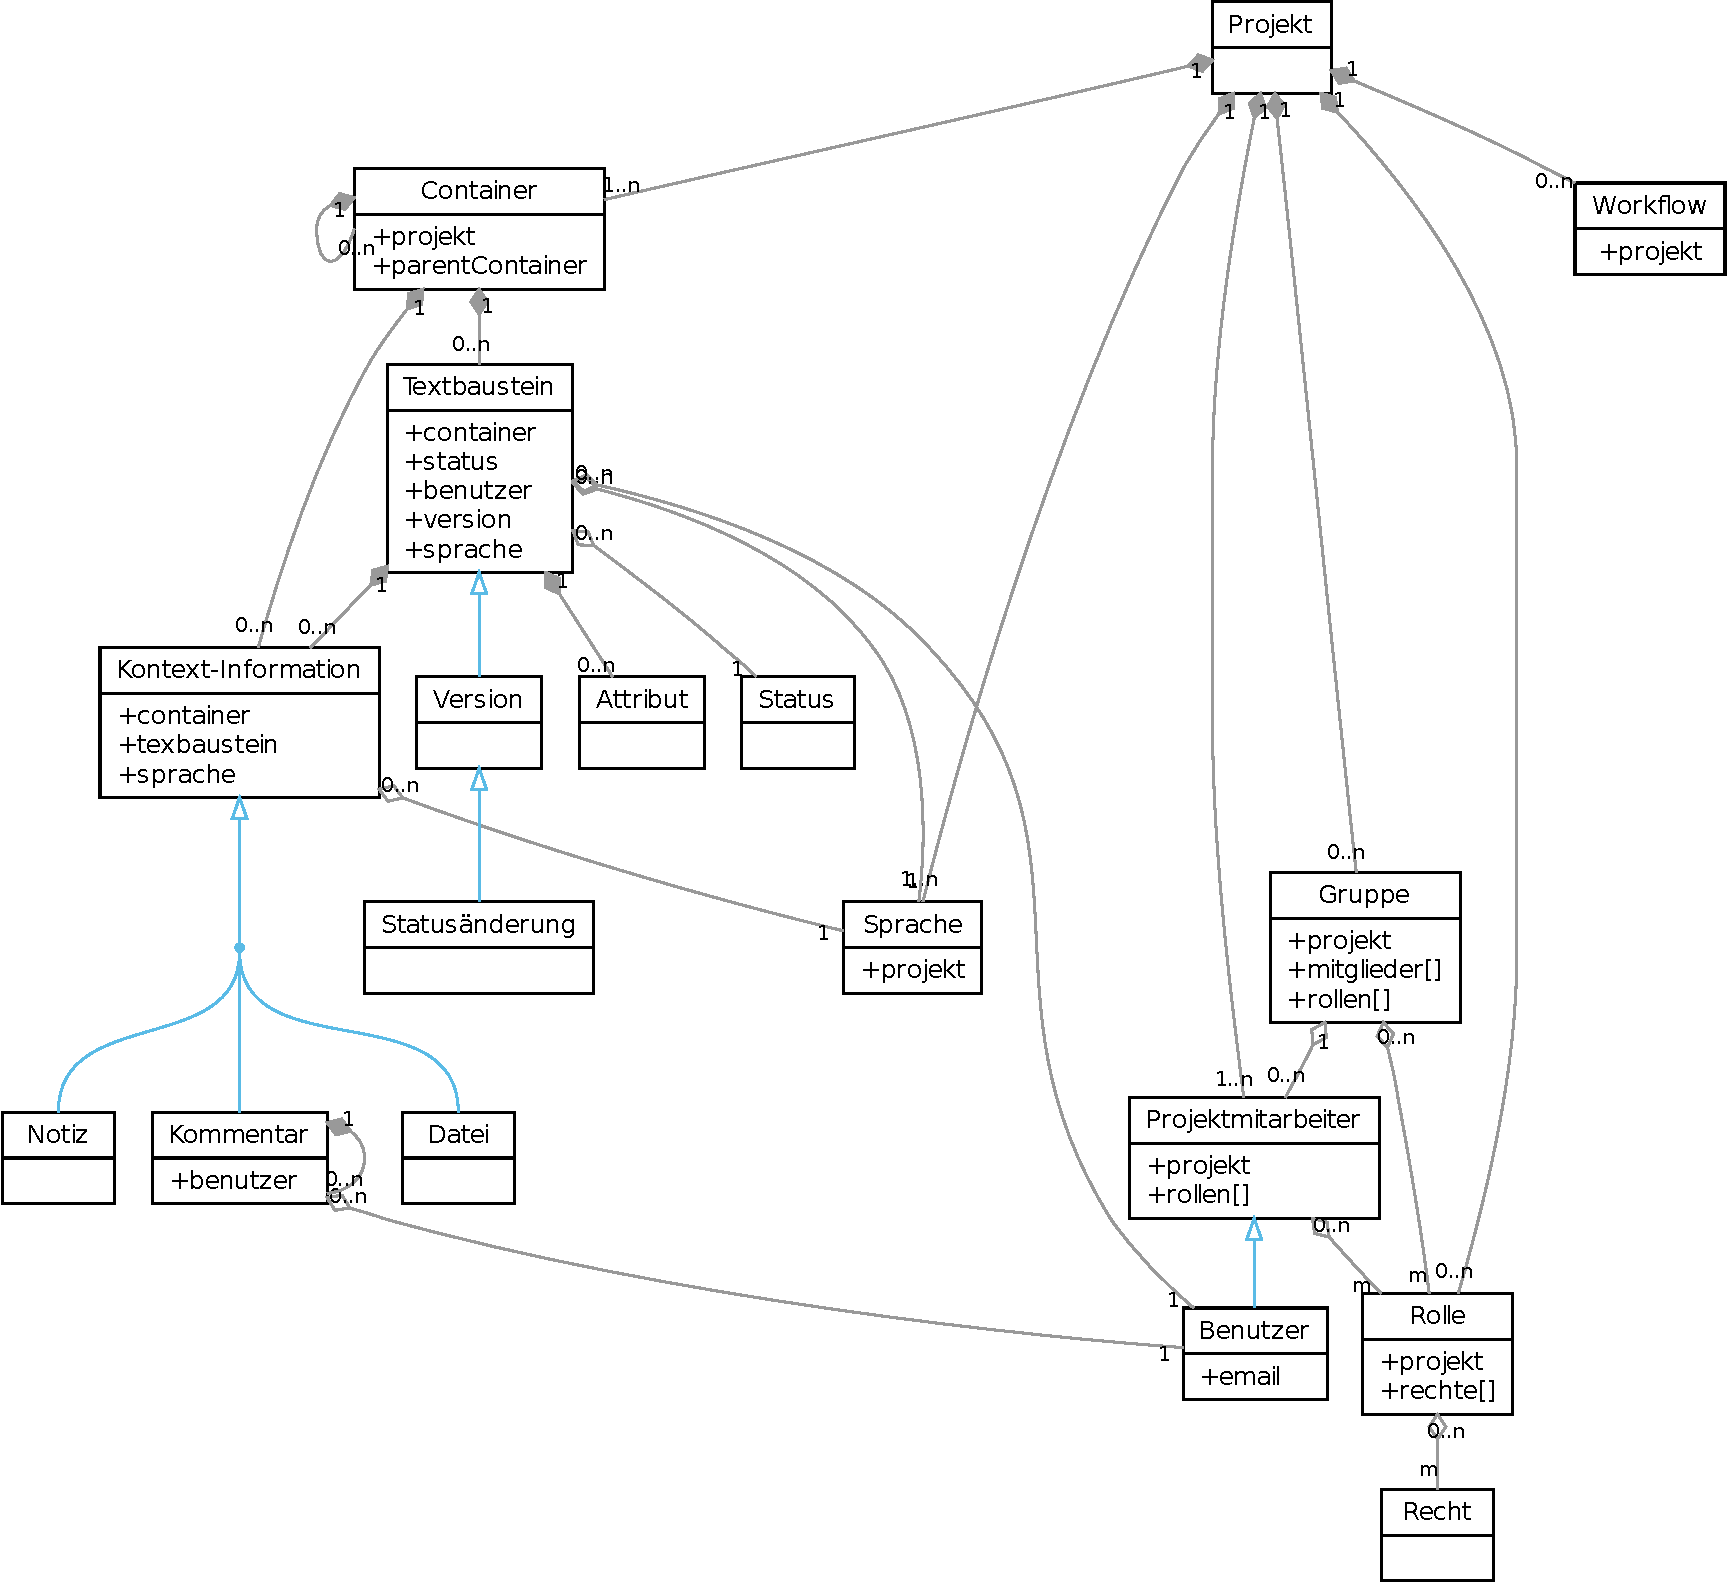
\includegraphics[width=\textwidth]{media/domain.pdf}
\captionof{figure}{Domänenmodell}\label{chart:domain}
\end{center}

Aus den vorangegangenen Überlegungen zur Anwendung und zum Workflow lässt sich ein Domänenmodell extrahieren, die einzelnen logischen Objekte innerhalb der Anwendung beschreibt, mit deren Hilfe alle Operationen abgebildet werden. Abbildung~\ref{chart:domain} zeigt das Modell in der Übersicht.

\subsubsection{Projekt}\label{model:projekt}

Projekte bildet den Rahmen für alle Texte eines einzelnen Produktes.

\subsubsection{Sprache}\label{model:sprache}

Die Texte jedes Projekts liegen in einer oder mehreren Sprachen vor.

\subsubsection{Container}\label{model:container}

Containern dienen zur hierarchischen Organisation der Texte innerhalb des Projektes. Containern können weitere Container und Texte enthalten. Eine Container ohne übergeordneten Container befindet sich auf der obersten Ebene. Es kann mehrere Containern auf der obersten Ebene geben.

\subsubsection{Textbaustein}\label{model:textbaustein}

Beschreibt einen einzelnen Textbaustein.

\subsubsection{Version}\label{model:version}

Beschreibt eine Version des Inhalts eines Textbausteins.

\subsubsection{Attribut}\label{model:attribut}

Beschreibt die Attribute eines Textbausteins.

\subsubsection{Status}\label{model:status}

Beschreibt die verschiedenen Zustände eines Textbausteins.

\begin{enumerate}\itemsep -5pt
\item \texttt{Neu}, Textbaustein erzeugt
\item \texttt{Leer}, Textbaustein definiert
\item \texttt{Befüllt}, Textbaustein mit Inhalt befüllt
\item \texttt{Korrigiert}, Orthografie geprüft
\item \texttt{Geprüft}, Inhalt geprüft (Qualitätsicherung)
\item \texttt{Freigegeben}, durch Kunden freigegeben
\item \texttt{Veröffentlicht}, in Produkt übernommen
\end{enumerate}

\subsubsection{Statusänderung}\label{model:statuschange}

Beschreibt eine Änderung eines Status durch einen Benutzer, z.B. durch Freigabe oder Überprüfung.

\subsubsection{Benutzer}\label{model:benutzer}

Repräsentiert einen Benutzer des Systems

\subsubsection{Projektmitarbeiter}\label{model:projektmitarbeiter}

Gestattet einem Benutzer die Mitarbeit an einem Projekt und legt dabei fest, welche Rechte dem Benutzer für das Projekt zustehen.

\subsubsection{Kontext-Information}\label{model:contextinfo}

Projektspezifische Kontext-Informationen lassen sich hinterlegen und Textbausteinen und Containern zuordnen.

\subsubsection{Kommentare}\label{model:notizen}

Kommentare enthalten Hinweise und Fragen zu einzelnen Texten und Texbausteinen.

\subsubsection{Workflow}\label{model:workflow}

Beschreibt einen projektspezifischen Workflow.



\subsubsection{Rolle}\label{model:rolle}

Beschreibt die verschiedenen Rollen innerhalb der Anwendung. Die Rechte der Rollen sind durch die Zuordnung von Benutzern zu Projekten durch den Projektmitarbeiter immer an das jeweilige Projekt gebunden.

\begin{enumerate}\itemsep -5pt
\item \texttt{Administrator}, hat alle Rechte 
\end{enumerate}

\subsubsection{Recht}\label{model:recht}

Beschreibt ein Recht, eine Operation auf einem Objekt auszuführen. Die Rechte sind:

\begin{enumerate}\itemsep -5pt
\item \texttt{Create}, Erstellen eines Objekts
\item \texttt{Read}, Lesen eines Objekts
\item \texttt{Update}, Modifizieren eines Objekts
\item \texttt{Delete}, Löschen eines Objekts
\end{enumerate}

\subsubsection{Gruppe}\label{model:gruppe}

Mitarbeiter können in Gruppen zusammengefasst werden. Dies erleichtert die Konfiguration des Workflows und der Rechte.